% Created by tikzDevice version 0.12.6 on 2025-02-14 03:21:45
% !TEX encoding = UTF-8 Unicode
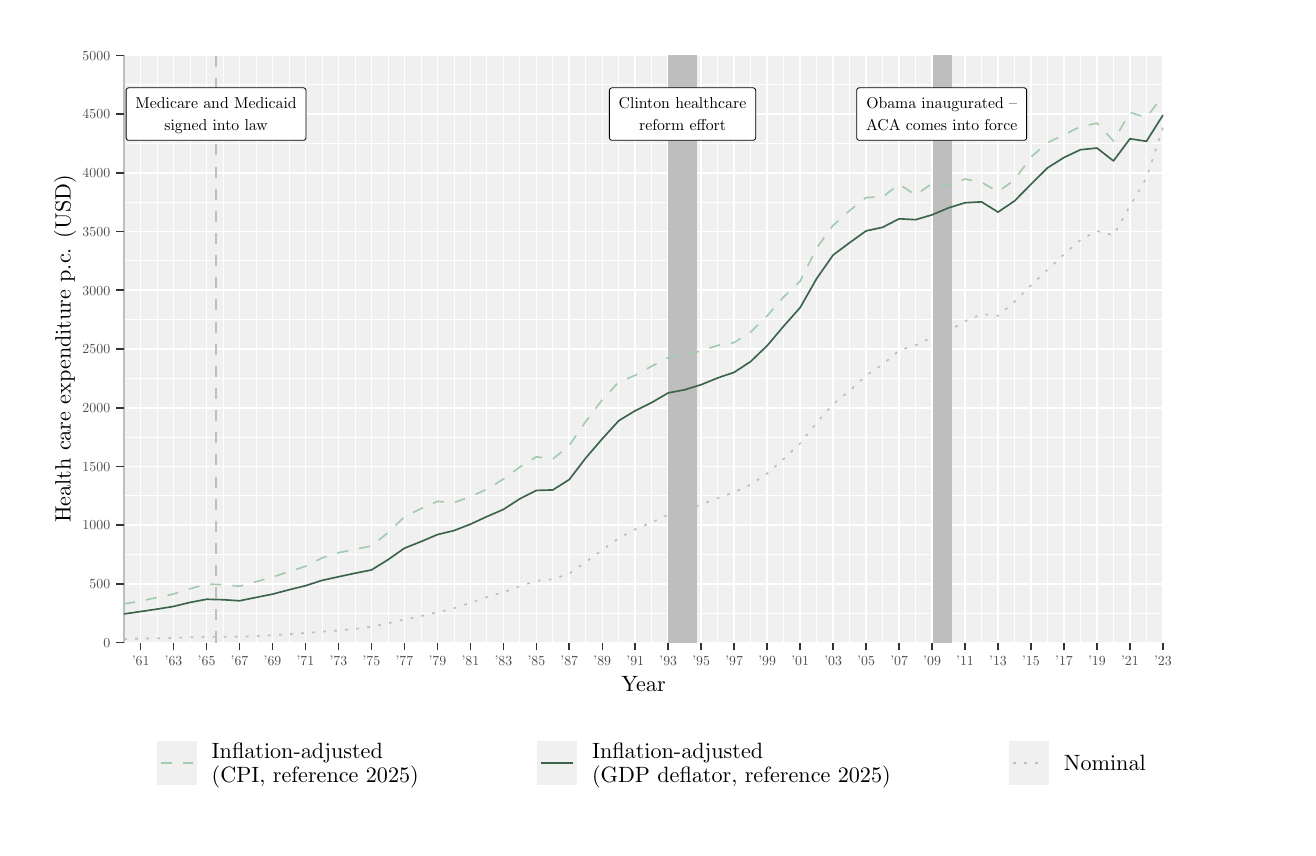
\begin{tikzpicture}[x=1pt,y=1pt]
\definecolor{fillColor}{RGB}{255,255,255}
\path[use as bounding box,fill=fillColor,fill opacity=0.00] (0,0) rectangle (455.30,289.08);
\begin{scope}
\path[clip] (  0.00,  0.00) rectangle (455.30,289.08);
\definecolor{drawColor}{RGB}{255,255,255}
\definecolor{fillColor}{RGB}{255,255,255}

\path[draw=drawColor,line width= 0.6pt,line join=round,line cap=round,fill=fillColor] ( -0.00,  0.00) rectangle (455.30,289.08);
\end{scope}
\begin{scope}
\path[clip] (  0.00,  0.00) rectangle (455.30,289.08);
\definecolor{fillColor}{gray}{0.94}

\path[fill=fillColor] ( 34.76, 66.89) rectangle (410.30,279.08);
\definecolor{drawColor}{RGB}{255,255,255}

\path[draw=drawColor,line width= 0.3pt,line join=round] ( 34.76, 77.50) --
	(410.30, 77.50);

\path[draw=drawColor,line width= 0.3pt,line join=round] ( 34.76, 98.71) --
	(410.30, 98.71);

\path[draw=drawColor,line width= 0.3pt,line join=round] ( 34.76,119.93) --
	(410.30,119.93);

\path[draw=drawColor,line width= 0.3pt,line join=round] ( 34.76,141.15) --
	(410.30,141.15);

\path[draw=drawColor,line width= 0.3pt,line join=round] ( 34.76,162.37) --
	(410.30,162.37);

\path[draw=drawColor,line width= 0.3pt,line join=round] ( 34.76,183.59) --
	(410.30,183.59);

\path[draw=drawColor,line width= 0.3pt,line join=round] ( 34.76,204.81) --
	(410.30,204.81);

\path[draw=drawColor,line width= 0.3pt,line join=round] ( 34.76,226.03) --
	(410.30,226.03);

\path[draw=drawColor,line width= 0.3pt,line join=round] ( 34.76,247.25) --
	(410.30,247.25);

\path[draw=drawColor,line width= 0.3pt,line join=round] ( 34.76,268.47) --
	(410.30,268.47);

\path[draw=drawColor,line width= 0.3pt,line join=round] ( 34.85, 66.89) --
	( 34.85,279.08);

\path[draw=drawColor,line width= 0.3pt,line join=round] ( 46.77, 66.89) --
	( 46.77,279.08);

\path[draw=drawColor,line width= 0.3pt,line join=round] ( 58.69, 66.89) --
	( 58.69,279.08);

\path[draw=drawColor,line width= 0.3pt,line join=round] ( 70.60, 66.89) --
	( 70.60,279.08);

\path[draw=drawColor,line width= 0.3pt,line join=round] ( 82.52, 66.89) --
	( 82.52,279.08);

\path[draw=drawColor,line width= 0.3pt,line join=round] ( 94.43, 66.89) --
	( 94.43,279.08);

\path[draw=drawColor,line width= 0.3pt,line join=round] (106.35, 66.89) --
	(106.35,279.08);

\path[draw=drawColor,line width= 0.3pt,line join=round] (118.27, 66.89) --
	(118.27,279.08);

\path[draw=drawColor,line width= 0.3pt,line join=round] (130.18, 66.89) --
	(130.18,279.08);

\path[draw=drawColor,line width= 0.3pt,line join=round] (142.10, 66.89) --
	(142.10,279.08);

\path[draw=drawColor,line width= 0.3pt,line join=round] (154.02, 66.89) --
	(154.02,279.08);

\path[draw=drawColor,line width= 0.3pt,line join=round] (165.93, 66.89) --
	(165.93,279.08);

\path[draw=drawColor,line width= 0.3pt,line join=round] (177.85, 66.89) --
	(177.85,279.08);

\path[draw=drawColor,line width= 0.3pt,line join=round] (189.77, 66.89) --
	(189.77,279.08);

\path[draw=drawColor,line width= 0.3pt,line join=round] (201.68, 66.89) --
	(201.68,279.08);

\path[draw=drawColor,line width= 0.3pt,line join=round] (213.60, 66.89) --
	(213.60,279.08);

\path[draw=drawColor,line width= 0.3pt,line join=round] (225.52, 66.89) --
	(225.52,279.08);

\path[draw=drawColor,line width= 0.3pt,line join=round] (237.43, 66.89) --
	(237.43,279.08);

\path[draw=drawColor,line width= 0.3pt,line join=round] (249.35, 66.89) --
	(249.35,279.08);

\path[draw=drawColor,line width= 0.3pt,line join=round] (261.27, 66.89) --
	(261.27,279.08);

\path[draw=drawColor,line width= 0.3pt,line join=round] (273.18, 66.89) --
	(273.18,279.08);

\path[draw=drawColor,line width= 0.3pt,line join=round] (285.10, 66.89) --
	(285.10,279.08);

\path[draw=drawColor,line width= 0.3pt,line join=round] (297.02, 66.89) --
	(297.02,279.08);

\path[draw=drawColor,line width= 0.3pt,line join=round] (308.93, 66.89) --
	(308.93,279.08);

\path[draw=drawColor,line width= 0.3pt,line join=round] (320.85, 66.89) --
	(320.85,279.08);

\path[draw=drawColor,line width= 0.3pt,line join=round] (332.77, 66.89) --
	(332.77,279.08);

\path[draw=drawColor,line width= 0.3pt,line join=round] (344.68, 66.89) --
	(344.68,279.08);

\path[draw=drawColor,line width= 0.3pt,line join=round] (356.60, 66.89) --
	(356.60,279.08);

\path[draw=drawColor,line width= 0.3pt,line join=round] (368.52, 66.89) --
	(368.52,279.08);

\path[draw=drawColor,line width= 0.3pt,line join=round] (380.43, 66.89) --
	(380.43,279.08);

\path[draw=drawColor,line width= 0.3pt,line join=round] (392.35, 66.89) --
	(392.35,279.08);

\path[draw=drawColor,line width= 0.3pt,line join=round] (404.27, 66.89) --
	(404.27,279.08);

\path[draw=drawColor,line width= 0.6pt,line join=round] ( 34.76, 66.89) --
	(410.30, 66.89);

\path[draw=drawColor,line width= 0.6pt,line join=round] ( 34.76, 88.10) --
	(410.30, 88.10);

\path[draw=drawColor,line width= 0.6pt,line join=round] ( 34.76,109.32) --
	(410.30,109.32);

\path[draw=drawColor,line width= 0.6pt,line join=round] ( 34.76,130.54) --
	(410.30,130.54);

\path[draw=drawColor,line width= 0.6pt,line join=round] ( 34.76,151.76) --
	(410.30,151.76);

\path[draw=drawColor,line width= 0.6pt,line join=round] ( 34.76,172.98) --
	(410.30,172.98);

\path[draw=drawColor,line width= 0.6pt,line join=round] ( 34.76,194.20) --
	(410.30,194.20);

\path[draw=drawColor,line width= 0.6pt,line join=round] ( 34.76,215.42) --
	(410.30,215.42);

\path[draw=drawColor,line width= 0.6pt,line join=round] ( 34.76,236.64) --
	(410.30,236.64);

\path[draw=drawColor,line width= 0.6pt,line join=round] ( 34.76,257.86) --
	(410.30,257.86);

\path[draw=drawColor,line width= 0.6pt,line join=round] ( 34.76,279.08) --
	(410.30,279.08);

\path[draw=drawColor,line width= 0.6pt,line join=round] ( 40.81, 66.89) --
	( 40.81,279.08);

\path[draw=drawColor,line width= 0.6pt,line join=round] ( 52.72, 66.89) --
	( 52.72,279.08);

\path[draw=drawColor,line width= 0.6pt,line join=round] ( 64.65, 66.89) --
	( 64.65,279.08);

\path[draw=drawColor,line width= 0.6pt,line join=round] ( 76.56, 66.89) --
	( 76.56,279.08);

\path[draw=drawColor,line width= 0.6pt,line join=round] ( 88.48, 66.89) --
	( 88.48,279.08);

\path[draw=drawColor,line width= 0.6pt,line join=round] (100.39, 66.89) --
	(100.39,279.08);

\path[draw=drawColor,line width= 0.6pt,line join=round] (112.31, 66.89) --
	(112.31,279.08);

\path[draw=drawColor,line width= 0.6pt,line join=round] (124.22, 66.89) --
	(124.22,279.08);

\path[draw=drawColor,line width= 0.6pt,line join=round] (136.15, 66.89) --
	(136.15,279.08);

\path[draw=drawColor,line width= 0.6pt,line join=round] (148.06, 66.89) --
	(148.06,279.08);

\path[draw=drawColor,line width= 0.6pt,line join=round] (159.98, 66.89) --
	(159.98,279.08);

\path[draw=drawColor,line width= 0.6pt,line join=round] (171.89, 66.89) --
	(171.89,279.08);

\path[draw=drawColor,line width= 0.6pt,line join=round] (183.81, 66.89) --
	(183.81,279.08);

\path[draw=drawColor,line width= 0.6pt,line join=round] (195.72, 66.89) --
	(195.72,279.08);

\path[draw=drawColor,line width= 0.6pt,line join=round] (207.65, 66.89) --
	(207.65,279.08);

\path[draw=drawColor,line width= 0.6pt,line join=round] (219.55, 66.89) --
	(219.55,279.08);

\path[draw=drawColor,line width= 0.6pt,line join=round] (231.48, 66.89) --
	(231.48,279.08);

\path[draw=drawColor,line width= 0.6pt,line join=round] (243.39, 66.89) --
	(243.39,279.08);

\path[draw=drawColor,line width= 0.6pt,line join=round] (255.31, 66.89) --
	(255.31,279.08);

\path[draw=drawColor,line width= 0.6pt,line join=round] (267.22, 66.89) --
	(267.22,279.08);

\path[draw=drawColor,line width= 0.6pt,line join=round] (279.15, 66.89) --
	(279.15,279.08);

\path[draw=drawColor,line width= 0.6pt,line join=round] (291.05, 66.89) --
	(291.05,279.08);

\path[draw=drawColor,line width= 0.6pt,line join=round] (302.98, 66.89) --
	(302.98,279.08);

\path[draw=drawColor,line width= 0.6pt,line join=round] (314.89, 66.89) --
	(314.89,279.08);

\path[draw=drawColor,line width= 0.6pt,line join=round] (326.81, 66.89) --
	(326.81,279.08);

\path[draw=drawColor,line width= 0.6pt,line join=round] (338.72, 66.89) --
	(338.72,279.08);

\path[draw=drawColor,line width= 0.6pt,line join=round] (350.64, 66.89) --
	(350.64,279.08);

\path[draw=drawColor,line width= 0.6pt,line join=round] (362.55, 66.89) --
	(362.55,279.08);

\path[draw=drawColor,line width= 0.6pt,line join=round] (374.48, 66.89) --
	(374.48,279.08);

\path[draw=drawColor,line width= 0.6pt,line join=round] (386.39, 66.89) --
	(386.39,279.08);

\path[draw=drawColor,line width= 0.6pt,line join=round] (398.31, 66.89) --
	(398.31,279.08);

\path[draw=drawColor,line width= 0.6pt,line join=round] (410.22, 66.89) --
	(410.22,279.08);
\definecolor{drawColor}{RGB}{190,190,190}

\path[draw=drawColor,line width= 0.6pt,line join=round] ( 34.84, 66.89) -- ( 34.84,279.08);
\definecolor{fillColor}{RGB}{190,190,190}

\path[fill=fillColor,fill opacity=0.01] (231.48, 66.89) rectangle (241.81,279.08);

\path[fill=fillColor,fill opacity=0.01] (231.48, 66.89) rectangle (241.81,279.08);

\path[fill=fillColor,fill opacity=0.01] (231.48, 66.89) rectangle (241.81,279.08);

\path[fill=fillColor,fill opacity=0.01] (231.48, 66.89) rectangle (241.81,279.08);

\path[fill=fillColor,fill opacity=0.01] (231.48, 66.89) rectangle (241.81,279.08);

\path[fill=fillColor,fill opacity=0.01] (231.48, 66.89) rectangle (241.81,279.08);

\path[fill=fillColor,fill opacity=0.01] (231.48, 66.89) rectangle (241.81,279.08);

\path[fill=fillColor,fill opacity=0.01] (231.48, 66.89) rectangle (241.81,279.08);

\path[fill=fillColor,fill opacity=0.01] (231.48, 66.89) rectangle (241.81,279.08);

\path[fill=fillColor,fill opacity=0.01] (231.48, 66.89) rectangle (241.81,279.08);

\path[fill=fillColor,fill opacity=0.01] (231.48, 66.89) rectangle (241.81,279.08);

\path[fill=fillColor,fill opacity=0.01] (231.48, 66.89) rectangle (241.81,279.08);

\path[fill=fillColor,fill opacity=0.01] (231.48, 66.89) rectangle (241.81,279.08);

\path[fill=fillColor,fill opacity=0.01] (231.48, 66.89) rectangle (241.81,279.08);

\path[fill=fillColor,fill opacity=0.01] (231.48, 66.89) rectangle (241.81,279.08);

\path[fill=fillColor,fill opacity=0.01] (231.48, 66.89) rectangle (241.81,279.08);

\path[fill=fillColor,fill opacity=0.01] (231.48, 66.89) rectangle (241.81,279.08);

\path[fill=fillColor,fill opacity=0.01] (231.48, 66.89) rectangle (241.81,279.08);

\path[fill=fillColor,fill opacity=0.01] (231.48, 66.89) rectangle (241.81,279.08);

\path[fill=fillColor,fill opacity=0.01] (231.48, 66.89) rectangle (241.81,279.08);

\path[fill=fillColor,fill opacity=0.01] (231.48, 66.89) rectangle (241.81,279.08);

\path[fill=fillColor,fill opacity=0.01] (231.48, 66.89) rectangle (241.81,279.08);

\path[fill=fillColor,fill opacity=0.01] (231.48, 66.89) rectangle (241.81,279.08);

\path[fill=fillColor,fill opacity=0.01] (231.48, 66.89) rectangle (241.81,279.08);

\path[fill=fillColor,fill opacity=0.01] (231.48, 66.89) rectangle (241.81,279.08);

\path[fill=fillColor,fill opacity=0.01] (231.48, 66.89) rectangle (241.81,279.08);

\path[fill=fillColor,fill opacity=0.01] (231.48, 66.89) rectangle (241.81,279.08);

\path[fill=fillColor,fill opacity=0.01] (231.48, 66.89) rectangle (241.81,279.08);

\path[fill=fillColor,fill opacity=0.01] (231.48, 66.89) rectangle (241.81,279.08);

\path[fill=fillColor,fill opacity=0.01] (231.48, 66.89) rectangle (241.81,279.08);

\path[fill=fillColor,fill opacity=0.01] (231.48, 66.89) rectangle (241.81,279.08);

\path[fill=fillColor,fill opacity=0.01] (231.48, 66.89) rectangle (241.81,279.08);

\path[fill=fillColor,fill opacity=0.01] (231.48, 66.89) rectangle (241.81,279.08);

\path[fill=fillColor,fill opacity=0.01] (231.48, 66.89) rectangle (241.81,279.08);

\path[fill=fillColor,fill opacity=0.01] (231.48, 66.89) rectangle (241.81,279.08);

\path[fill=fillColor,fill opacity=0.01] (231.48, 66.89) rectangle (241.81,279.08);

\path[fill=fillColor,fill opacity=0.01] (231.48, 66.89) rectangle (241.81,279.08);

\path[fill=fillColor,fill opacity=0.01] (231.48, 66.89) rectangle (241.81,279.08);

\path[fill=fillColor,fill opacity=0.01] (231.48, 66.89) rectangle (241.81,279.08);

\path[fill=fillColor,fill opacity=0.01] (231.48, 66.89) rectangle (241.81,279.08);

\path[fill=fillColor,fill opacity=0.01] (231.48, 66.89) rectangle (241.81,279.08);

\path[fill=fillColor,fill opacity=0.01] (231.48, 66.89) rectangle (241.81,279.08);

\path[fill=fillColor,fill opacity=0.01] (231.48, 66.89) rectangle (241.81,279.08);

\path[fill=fillColor,fill opacity=0.01] (231.48, 66.89) rectangle (241.81,279.08);

\path[fill=fillColor,fill opacity=0.01] (231.48, 66.89) rectangle (241.81,279.08);

\path[fill=fillColor,fill opacity=0.01] (231.48, 66.89) rectangle (241.81,279.08);

\path[fill=fillColor,fill opacity=0.01] (231.48, 66.89) rectangle (241.81,279.08);

\path[fill=fillColor,fill opacity=0.01] (231.48, 66.89) rectangle (241.81,279.08);

\path[fill=fillColor,fill opacity=0.01] (231.48, 66.89) rectangle (241.81,279.08);

\path[fill=fillColor,fill opacity=0.01] (231.48, 66.89) rectangle (241.81,279.08);

\path[fill=fillColor,fill opacity=0.01] (231.48, 66.89) rectangle (241.81,279.08);

\path[fill=fillColor,fill opacity=0.01] (231.48, 66.89) rectangle (241.81,279.08);

\path[fill=fillColor,fill opacity=0.01] (231.48, 66.89) rectangle (241.81,279.08);

\path[fill=fillColor,fill opacity=0.01] (231.48, 66.89) rectangle (241.81,279.08);

\path[fill=fillColor,fill opacity=0.01] (231.48, 66.89) rectangle (241.81,279.08);

\path[fill=fillColor,fill opacity=0.01] (231.48, 66.89) rectangle (241.81,279.08);

\path[fill=fillColor,fill opacity=0.01] (231.48, 66.89) rectangle (241.81,279.08);

\path[fill=fillColor,fill opacity=0.01] (231.48, 66.89) rectangle (241.81,279.08);

\path[fill=fillColor,fill opacity=0.01] (231.48, 66.89) rectangle (241.81,279.08);

\path[fill=fillColor,fill opacity=0.01] (231.48, 66.89) rectangle (241.81,279.08);

\path[fill=fillColor,fill opacity=0.01] (231.48, 66.89) rectangle (241.81,279.08);

\path[fill=fillColor,fill opacity=0.01] (231.48, 66.89) rectangle (241.81,279.08);

\path[fill=fillColor,fill opacity=0.01] (231.48, 66.89) rectangle (241.81,279.08);

\path[fill=fillColor,fill opacity=0.01] (231.48, 66.89) rectangle (241.81,279.08);

\path[fill=fillColor,fill opacity=0.01] (327.12, 66.89) rectangle (334.09,279.08);

\path[fill=fillColor,fill opacity=0.01] (327.12, 66.89) rectangle (334.09,279.08);

\path[fill=fillColor,fill opacity=0.01] (327.12, 66.89) rectangle (334.09,279.08);

\path[fill=fillColor,fill opacity=0.01] (327.12, 66.89) rectangle (334.09,279.08);

\path[fill=fillColor,fill opacity=0.01] (327.12, 66.89) rectangle (334.09,279.08);

\path[fill=fillColor,fill opacity=0.01] (327.12, 66.89) rectangle (334.09,279.08);

\path[fill=fillColor,fill opacity=0.01] (327.12, 66.89) rectangle (334.09,279.08);

\path[fill=fillColor,fill opacity=0.01] (327.12, 66.89) rectangle (334.09,279.08);

\path[fill=fillColor,fill opacity=0.01] (327.12, 66.89) rectangle (334.09,279.08);

\path[fill=fillColor,fill opacity=0.01] (327.12, 66.89) rectangle (334.09,279.08);

\path[fill=fillColor,fill opacity=0.01] (327.12, 66.89) rectangle (334.09,279.08);

\path[fill=fillColor,fill opacity=0.01] (327.12, 66.89) rectangle (334.09,279.08);

\path[fill=fillColor,fill opacity=0.01] (327.12, 66.89) rectangle (334.09,279.08);

\path[fill=fillColor,fill opacity=0.01] (327.12, 66.89) rectangle (334.09,279.08);

\path[fill=fillColor,fill opacity=0.01] (327.12, 66.89) rectangle (334.09,279.08);

\path[fill=fillColor,fill opacity=0.01] (327.12, 66.89) rectangle (334.09,279.08);

\path[fill=fillColor,fill opacity=0.01] (327.12, 66.89) rectangle (334.09,279.08);

\path[fill=fillColor,fill opacity=0.01] (327.12, 66.89) rectangle (334.09,279.08);

\path[fill=fillColor,fill opacity=0.01] (327.12, 66.89) rectangle (334.09,279.08);

\path[fill=fillColor,fill opacity=0.01] (327.12, 66.89) rectangle (334.09,279.08);

\path[fill=fillColor,fill opacity=0.01] (327.12, 66.89) rectangle (334.09,279.08);

\path[fill=fillColor,fill opacity=0.01] (327.12, 66.89) rectangle (334.09,279.08);

\path[fill=fillColor,fill opacity=0.01] (327.12, 66.89) rectangle (334.09,279.08);

\path[fill=fillColor,fill opacity=0.01] (327.12, 66.89) rectangle (334.09,279.08);

\path[fill=fillColor,fill opacity=0.01] (327.12, 66.89) rectangle (334.09,279.08);

\path[fill=fillColor,fill opacity=0.01] (327.12, 66.89) rectangle (334.09,279.08);

\path[fill=fillColor,fill opacity=0.01] (327.12, 66.89) rectangle (334.09,279.08);

\path[fill=fillColor,fill opacity=0.01] (327.12, 66.89) rectangle (334.09,279.08);

\path[fill=fillColor,fill opacity=0.01] (327.12, 66.89) rectangle (334.09,279.08);

\path[fill=fillColor,fill opacity=0.01] (327.12, 66.89) rectangle (334.09,279.08);

\path[fill=fillColor,fill opacity=0.01] (327.12, 66.89) rectangle (334.09,279.08);

\path[fill=fillColor,fill opacity=0.01] (327.12, 66.89) rectangle (334.09,279.08);

\path[fill=fillColor,fill opacity=0.01] (327.12, 66.89) rectangle (334.09,279.08);

\path[fill=fillColor,fill opacity=0.01] (327.12, 66.89) rectangle (334.09,279.08);

\path[fill=fillColor,fill opacity=0.01] (327.12, 66.89) rectangle (334.09,279.08);

\path[fill=fillColor,fill opacity=0.01] (327.12, 66.89) rectangle (334.09,279.08);

\path[fill=fillColor,fill opacity=0.01] (327.12, 66.89) rectangle (334.09,279.08);

\path[fill=fillColor,fill opacity=0.01] (327.12, 66.89) rectangle (334.09,279.08);

\path[fill=fillColor,fill opacity=0.01] (327.12, 66.89) rectangle (334.09,279.08);

\path[fill=fillColor,fill opacity=0.01] (327.12, 66.89) rectangle (334.09,279.08);

\path[fill=fillColor,fill opacity=0.01] (327.12, 66.89) rectangle (334.09,279.08);

\path[fill=fillColor,fill opacity=0.01] (327.12, 66.89) rectangle (334.09,279.08);

\path[fill=fillColor,fill opacity=0.01] (327.12, 66.89) rectangle (334.09,279.08);

\path[fill=fillColor,fill opacity=0.01] (327.12, 66.89) rectangle (334.09,279.08);

\path[fill=fillColor,fill opacity=0.01] (327.12, 66.89) rectangle (334.09,279.08);

\path[fill=fillColor,fill opacity=0.01] (327.12, 66.89) rectangle (334.09,279.08);

\path[fill=fillColor,fill opacity=0.01] (327.12, 66.89) rectangle (334.09,279.08);

\path[fill=fillColor,fill opacity=0.01] (327.12, 66.89) rectangle (334.09,279.08);

\path[fill=fillColor,fill opacity=0.01] (327.12, 66.89) rectangle (334.09,279.08);

\path[fill=fillColor,fill opacity=0.01] (327.12, 66.89) rectangle (334.09,279.08);

\path[fill=fillColor,fill opacity=0.01] (327.12, 66.89) rectangle (334.09,279.08);

\path[fill=fillColor,fill opacity=0.01] (327.12, 66.89) rectangle (334.09,279.08);

\path[fill=fillColor,fill opacity=0.01] (327.12, 66.89) rectangle (334.09,279.08);

\path[fill=fillColor,fill opacity=0.01] (327.12, 66.89) rectangle (334.09,279.08);

\path[fill=fillColor,fill opacity=0.01] (327.12, 66.89) rectangle (334.09,279.08);

\path[fill=fillColor,fill opacity=0.01] (327.12, 66.89) rectangle (334.09,279.08);

\path[fill=fillColor,fill opacity=0.01] (327.12, 66.89) rectangle (334.09,279.08);

\path[fill=fillColor,fill opacity=0.01] (327.12, 66.89) rectangle (334.09,279.08);

\path[fill=fillColor,fill opacity=0.01] (327.12, 66.89) rectangle (334.09,279.08);

\path[fill=fillColor,fill opacity=0.01] (327.12, 66.89) rectangle (334.09,279.08);

\path[fill=fillColor,fill opacity=0.01] (327.12, 66.89) rectangle (334.09,279.08);

\path[fill=fillColor,fill opacity=0.01] (327.12, 66.89) rectangle (334.09,279.08);

\path[fill=fillColor,fill opacity=0.01] (327.12, 66.89) rectangle (334.09,279.08);

\path[fill=fillColor,fill opacity=0.01] (327.12, 66.89) rectangle (334.09,279.08);

\path[draw=drawColor,line width= 0.6pt,dash pattern=on 4pt off 4pt ,line join=round] ( 68.07, 66.89) -- ( 68.07,279.08);
\definecolor{drawColor}{RGB}{0,0,0}
\definecolor{fillColor}{RGB}{255,255,255}

\path[draw=drawColor,line width= 0.3pt,line join=round,line cap=round,fill=fillColor] ( 36.59,248.38) --
	( 99.56,248.38) --
	( 99.52,248.38) --
	( 99.68,248.38) --
	( 99.85,248.42) --
	(100.00,248.48) --
	(100.14,248.56) --
	(100.27,248.66) --
	(100.38,248.79) --
	(100.47,248.93) --
	(100.54,249.08) --
	(100.58,249.24) --
	(100.59,249.40) --
	(100.59,249.40) --
	(100.59,266.32) --
	(100.59,266.32) --
	(100.58,266.48) --
	(100.54,266.64) --
	(100.47,266.79) --
	(100.38,266.93) --
	(100.27,267.06) --
	(100.14,267.16) --
	(100.00,267.25) --
	( 99.85,267.30) --
	( 99.68,267.34) --
	( 99.56,267.34) --
	( 36.59,267.34) --
	( 36.71,267.34) --
	( 36.54,267.34) --
	( 36.38,267.32) --
	( 36.22,267.28) --
	( 36.07,267.21) --
	( 35.94,267.11) --
	( 35.82,267.00) --
	( 35.72,266.87) --
	( 35.64,266.72) --
	( 35.59,266.56) --
	( 35.56,266.40) --
	( 35.56,266.32) --
	( 35.56,249.40) --
	( 35.56,249.49) --
	( 35.56,249.32) --
	( 35.59,249.16) --
	( 35.64,249.00) --
	( 35.72,248.86) --
	( 35.82,248.72) --
	( 35.94,248.61) --
	( 36.07,248.51) --
	( 36.22,248.44) --
	( 36.38,248.40) --
	( 36.54,248.38) --
	cycle;
\end{scope}
\begin{scope}
\path[clip] (  0.00,  0.00) rectangle (455.30,289.08);
\definecolor{drawColor}{RGB}{0,0,0}

\node[text=drawColor,anchor=base,inner sep=0pt, outer sep=0pt, scale=  0.57] at ( 68.07,260.00) {Medicare and Medicaid };

\node[text=drawColor,anchor=base,inner sep=0pt, outer sep=0pt, scale=  0.57] at ( 68.07,251.80) { signed into law};
\end{scope}
\begin{scope}
\path[clip] (  0.00,  0.00) rectangle (455.30,289.08);
\definecolor{drawColor}{RGB}{0,0,0}
\definecolor{fillColor}{RGB}{255,255,255}

\path[draw=drawColor,line width= 0.3pt,line join=round,line cap=round,fill=fillColor] (211.23,248.38) --
	(262.04,248.38) --
	(262.00,248.38) --
	(262.16,248.38) --
	(262.32,248.42) --
	(262.48,248.48) --
	(262.62,248.56) --
	(262.75,248.66) --
	(262.86,248.79) --
	(262.95,248.93) --
	(263.01,249.08) --
	(263.05,249.24) --
	(263.07,249.40) --
	(263.07,249.40) --
	(263.07,266.32) --
	(263.07,266.32) --
	(263.05,266.48) --
	(263.01,266.64) --
	(262.95,266.79) --
	(262.86,266.93) --
	(262.75,267.06) --
	(262.62,267.16) --
	(262.48,267.25) --
	(262.32,267.30) --
	(262.16,267.34) --
	(262.04,267.34) --
	(211.23,267.34) --
	(211.36,267.34) --
	(211.19,267.34) --
	(211.03,267.32) --
	(210.87,267.28) --
	(210.72,267.21) --
	(210.58,267.11) --
	(210.46,267.00) --
	(210.36,266.87) --
	(210.29,266.72) --
	(210.23,266.56) --
	(210.21,266.40) --
	(210.20,266.32) --
	(210.20,249.40) --
	(210.21,249.49) --
	(210.21,249.32) --
	(210.23,249.16) --
	(210.29,249.00) --
	(210.36,248.86) --
	(210.46,248.72) --
	(210.58,248.61) --
	(210.72,248.51) --
	(210.87,248.44) --
	(211.03,248.40) --
	(211.19,248.38) --
	cycle;
\end{scope}
\begin{scope}
\path[clip] (  0.00,  0.00) rectangle (455.30,289.08);
\definecolor{drawColor}{RGB}{0,0,0}

\node[text=drawColor,anchor=base,inner sep=0pt, outer sep=0pt, scale=  0.57] at (236.63,260.00) {Clinton healthcare };

\node[text=drawColor,anchor=base,inner sep=0pt, outer sep=0pt, scale=  0.57] at (236.63,251.80) { reform effort};
\end{scope}
\begin{scope}
\path[clip] (  0.00,  0.00) rectangle (455.30,289.08);
\definecolor{drawColor}{RGB}{0,0,0}
\definecolor{fillColor}{RGB}{255,255,255}

\path[draw=drawColor,line width= 0.3pt,line join=round,line cap=round,fill=fillColor] (300.58,248.38) --
	(359.96,248.38) --
	(359.91,248.38) --
	(360.08,248.38) --
	(360.24,248.42) --
	(360.40,248.48) --
	(360.54,248.56) --
	(360.67,248.66) --
	(360.78,248.79) --
	(360.87,248.93) --
	(360.93,249.08) --
	(360.97,249.24) --
	(360.98,249.40) --
	(360.98,249.40) --
	(360.98,266.32) --
	(360.98,266.32) --
	(360.97,266.48) --
	(360.93,266.64) --
	(360.87,266.79) --
	(360.78,266.93) --
	(360.67,267.06) --
	(360.54,267.16) --
	(360.40,267.25) --
	(360.24,267.30) --
	(360.08,267.34) --
	(359.96,267.34) --
	(300.58,267.34) --
	(300.71,267.34) --
	(300.54,267.34) --
	(300.38,267.32) --
	(300.22,267.28) --
	(300.07,267.21) --
	(299.93,267.11) --
	(299.81,267.00) --
	(299.72,266.87) --
	(299.64,266.72) --
	(299.59,266.56) --
	(299.56,266.40) --
	(299.56,266.32) --
	(299.56,249.40) --
	(299.56,249.49) --
	(299.56,249.32) --
	(299.59,249.16) --
	(299.64,249.00) --
	(299.72,248.86) --
	(299.81,248.72) --
	(299.93,248.61) --
	(300.07,248.51) --
	(300.22,248.44) --
	(300.38,248.40) --
	(300.54,248.38) --
	cycle;
\end{scope}
\begin{scope}
\path[clip] (  0.00,  0.00) rectangle (455.30,289.08);
\definecolor{drawColor}{RGB}{0,0,0}

\node[text=drawColor,anchor=base,inner sep=0pt, outer sep=0pt, scale=  0.57] at (330.27,260.00) {Obama inaugurated -- };

\node[text=drawColor,anchor=base,inner sep=0pt, outer sep=0pt, scale=  0.57] at (330.27,251.80) { ACA comes into force};
\end{scope}
\begin{scope}
\path[clip] (  0.00,  0.00) rectangle (455.30,289.08);
\definecolor{drawColor}{RGB}{190,190,190}

\path[draw=drawColor,line width= 0.6pt,dash pattern=on 1pt off 3pt ,line join=round] ( 34.84, 68.17) --
	( 40.81, 68.29) --
	( 46.77, 68.42) --
	( 52.72, 68.57) --
	( 58.68, 68.78) --
	( 64.65, 68.96) --
	( 70.60, 68.98) --
	( 76.56, 68.99) --
	( 82.51, 69.25) --
	( 88.48, 69.54) --
	( 94.43, 69.93) --
	(100.39, 70.34) --
	(106.34, 70.84) --
	(112.31, 71.24) --
	(118.27, 71.82) --
	(124.22, 72.62) --
	(130.18, 73.83) --
	(136.15, 75.25) --
	(142.10, 76.41) --
	(148.06, 77.85) --
	(154.01, 79.27) --
	(159.98, 81.32) --
	(165.93, 83.34) --
	(171.89, 85.07) --
	(177.84, 87.24) --
	(183.81, 89.18) --
	(189.77, 89.77) --
	(195.72, 91.82) --
	(201.68, 95.99) --
	(207.65,100.34) --
	(213.60,104.63) --
	(219.55,107.81) --
	(225.51,110.31) --
	(231.48,113.12) --
	(237.43,114.74) --
	(243.39,116.77) --
	(249.34,119.07) --
	(255.31,121.18) --
	(261.27,123.98) --
	(267.22,127.97) --
	(273.18,133.25) --
	(279.15,138.87) --
	(285.10,146.37) --
	(291.05,153.12) --
	(297.01,157.88) --
	(302.98,163.43) --
	(308.93,167.38) --
	(314.89,172.43) --
	(320.84,174.34) --
	(326.81,177.11) --
	(332.77,179.53) --
	(338.72,183.01) --
	(344.67,185.56) --
	(350.64,184.97) --
	(356.60,190.00) --
	(362.55,195.95) --
	(368.51,201.58) --
	(374.48,207.20) --
	(380.43,212.36) --
	(386.39,215.60) --
	(392.34,214.07) --
	(398.31,224.63) --
	(404.27,234.82) --
	(410.22,252.99);
\definecolor{drawColor}{RGB}{164,203,174}

\path[draw=drawColor,line width= 0.6pt,dash pattern=on 4pt off 4pt ,line join=round] ( 34.84, 80.84) --
	( 40.81, 81.91) --
	( 46.77, 83.18) --
	( 52.72, 84.44) --
	( 58.68, 86.36) --
	( 64.65, 88.00) --
	( 70.60, 87.83) --
	( 76.56, 87.24) --
	( 82.51, 88.88) --
	( 88.48, 90.53) --
	( 94.43, 92.49) --
	(100.39, 94.43) --
	(106.34, 97.44) --
	(112.31, 99.35) --
	(118.27,100.53) --
	(124.22,101.85) --
	(130.18,106.55) --
	(136.15,112.33) --
	(142.10,115.28) --
	(148.06,117.90) --
	(154.01,117.44) --
	(159.98,119.58) --
	(165.93,122.32) --
	(171.89,125.95) --
	(177.84,130.33) --
	(183.81,134.01) --
	(189.77,133.22) --
	(195.72,138.11) --
	(201.68,146.79) --
	(207.65,154.65) --
	(213.60,161.01) --
	(219.55,163.46) --
	(225.51,166.77) --
	(231.48,169.88) --
	(237.43,170.87) --
	(243.39,172.32) --
	(249.34,174.25) --
	(255.31,175.30) --
	(261.27,179.13) --
	(267.22,184.98) --
	(273.18,191.79) --
	(279.15,197.48) --
	(285.10,209.46) --
	(291.05,217.65) --
	(297.01,222.97) --
	(302.98,227.71) --
	(308.93,227.88) --
	(314.89,232.52) --
	(320.84,228.60) --
	(326.81,232.72) --
	(332.77,232.02) --
	(338.72,234.40) --
	(344.67,233.21) --
	(350.64,229.79) --
	(356.60,234.09) --
	(362.55,242.33) --
	(368.51,247.49) --
	(374.48,250.44) --
	(380.43,253.32) --
	(386.39,254.57) --
	(392.34,248.13) --
	(398.31,258.45) --
	(404.27,256.64) --
	(410.22,264.50);
\definecolor{drawColor}{RGB}{60,100,75}

\path[draw=drawColor,line width= 0.6pt,line join=round] ( 34.84, 77.24) --
	( 40.81, 78.10) --
	( 46.77, 78.98) --
	( 52.72, 79.95) --
	( 58.68, 81.40) --
	( 64.65, 82.53) --
	( 70.60, 82.37) --
	( 76.56, 81.98) --
	( 82.51, 83.19) --
	( 88.48, 84.39) --
	( 94.43, 85.96) --
	(100.39, 87.43) --
	(106.34, 89.35) --
	(112.31, 90.66) --
	(118.27, 91.94) --
	(124.22, 93.13) --
	(130.18, 96.82) --
	(136.15,100.99) --
	(142.10,103.36) --
	(148.06,105.90) --
	(154.01,107.34) --
	(159.98,109.66) --
	(165.93,112.41) --
	(171.89,114.99) --
	(177.84,118.84) --
	(183.81,121.86) --
	(189.77,122.04) --
	(195.72,125.80) --
	(201.68,133.61) --
	(207.65,140.54) --
	(213.60,147.07) --
	(219.55,150.67) --
	(225.51,153.62) --
	(231.48,157.11) --
	(237.43,158.23) --
	(243.39,160.09) --
	(249.34,162.52) --
	(255.31,164.55) --
	(261.27,168.46) --
	(267.22,174.18) --
	(273.18,181.22) --
	(279.15,187.95) --
	(285.10,198.43) --
	(291.05,206.92) --
	(297.01,211.38) --
	(302.98,215.65) --
	(308.93,216.94) --
	(314.89,220.02) --
	(320.84,219.69) --
	(326.81,221.45) --
	(332.77,223.97) --
	(338.72,225.81) --
	(344.67,226.14) --
	(350.64,222.44) --
	(356.60,226.47) --
	(362.55,232.49) --
	(368.51,238.42) --
	(374.48,242.17) --
	(380.43,244.98) --
	(386.39,245.58) --
	(392.34,240.93) --
	(398.31,248.93) --
	(404.27,248.02) --
	(410.22,257.46);
\end{scope}
\begin{scope}
\path[clip] (  0.00,  0.00) rectangle (455.30,289.08);
\definecolor{drawColor}{gray}{0.30}

\node[text=drawColor,anchor=base east,inner sep=0pt, outer sep=0pt, scale=  0.50] at ( 29.81, 65.16) {0};

\node[text=drawColor,anchor=base east,inner sep=0pt, outer sep=0pt, scale=  0.50] at ( 29.81, 86.38) {500};

\node[text=drawColor,anchor=base east,inner sep=0pt, outer sep=0pt, scale=  0.50] at ( 29.81,107.60) {1000};

\node[text=drawColor,anchor=base east,inner sep=0pt, outer sep=0pt, scale=  0.50] at ( 29.81,128.82) {1500};

\node[text=drawColor,anchor=base east,inner sep=0pt, outer sep=0pt, scale=  0.50] at ( 29.81,150.04) {2000};

\node[text=drawColor,anchor=base east,inner sep=0pt, outer sep=0pt, scale=  0.50] at ( 29.81,171.26) {2500};

\node[text=drawColor,anchor=base east,inner sep=0pt, outer sep=0pt, scale=  0.50] at ( 29.81,192.48) {3000};

\node[text=drawColor,anchor=base east,inner sep=0pt, outer sep=0pt, scale=  0.50] at ( 29.81,213.70) {3500};

\node[text=drawColor,anchor=base east,inner sep=0pt, outer sep=0pt, scale=  0.50] at ( 29.81,234.92) {4000};

\node[text=drawColor,anchor=base east,inner sep=0pt, outer sep=0pt, scale=  0.50] at ( 29.81,256.14) {4500};

\node[text=drawColor,anchor=base east,inner sep=0pt, outer sep=0pt, scale=  0.50] at ( 29.81,277.36) {5000};
\end{scope}
\begin{scope}
\path[clip] (  0.00,  0.00) rectangle (455.30,289.08);
\definecolor{drawColor}{gray}{0.20}

\path[draw=drawColor,line width= 0.6pt,line join=round] ( 32.01, 66.89) --
	( 34.76, 66.89);

\path[draw=drawColor,line width= 0.6pt,line join=round] ( 32.01, 88.10) --
	( 34.76, 88.10);

\path[draw=drawColor,line width= 0.6pt,line join=round] ( 32.01,109.32) --
	( 34.76,109.32);

\path[draw=drawColor,line width= 0.6pt,line join=round] ( 32.01,130.54) --
	( 34.76,130.54);

\path[draw=drawColor,line width= 0.6pt,line join=round] ( 32.01,151.76) --
	( 34.76,151.76);

\path[draw=drawColor,line width= 0.6pt,line join=round] ( 32.01,172.98) --
	( 34.76,172.98);

\path[draw=drawColor,line width= 0.6pt,line join=round] ( 32.01,194.20) --
	( 34.76,194.20);

\path[draw=drawColor,line width= 0.6pt,line join=round] ( 32.01,215.42) --
	( 34.76,215.42);

\path[draw=drawColor,line width= 0.6pt,line join=round] ( 32.01,236.64) --
	( 34.76,236.64);

\path[draw=drawColor,line width= 0.6pt,line join=round] ( 32.01,257.86) --
	( 34.76,257.86);

\path[draw=drawColor,line width= 0.6pt,line join=round] ( 32.01,279.08) --
	( 34.76,279.08);
\end{scope}
\begin{scope}
\path[clip] (  0.00,  0.00) rectangle (455.30,289.08);
\definecolor{drawColor}{gray}{0.20}

\path[draw=drawColor,line width= 0.6pt,line join=round] ( 40.81, 64.14) --
	( 40.81, 66.89);

\path[draw=drawColor,line width= 0.6pt,line join=round] ( 52.72, 64.14) --
	( 52.72, 66.89);

\path[draw=drawColor,line width= 0.6pt,line join=round] ( 64.65, 64.14) --
	( 64.65, 66.89);

\path[draw=drawColor,line width= 0.6pt,line join=round] ( 76.56, 64.14) --
	( 76.56, 66.89);

\path[draw=drawColor,line width= 0.6pt,line join=round] ( 88.48, 64.14) --
	( 88.48, 66.89);

\path[draw=drawColor,line width= 0.6pt,line join=round] (100.39, 64.14) --
	(100.39, 66.89);

\path[draw=drawColor,line width= 0.6pt,line join=round] (112.31, 64.14) --
	(112.31, 66.89);

\path[draw=drawColor,line width= 0.6pt,line join=round] (124.22, 64.14) --
	(124.22, 66.89);

\path[draw=drawColor,line width= 0.6pt,line join=round] (136.15, 64.14) --
	(136.15, 66.89);

\path[draw=drawColor,line width= 0.6pt,line join=round] (148.06, 64.14) --
	(148.06, 66.89);

\path[draw=drawColor,line width= 0.6pt,line join=round] (159.98, 64.14) --
	(159.98, 66.89);

\path[draw=drawColor,line width= 0.6pt,line join=round] (171.89, 64.14) --
	(171.89, 66.89);

\path[draw=drawColor,line width= 0.6pt,line join=round] (183.81, 64.14) --
	(183.81, 66.89);

\path[draw=drawColor,line width= 0.6pt,line join=round] (195.72, 64.14) --
	(195.72, 66.89);

\path[draw=drawColor,line width= 0.6pt,line join=round] (207.65, 64.14) --
	(207.65, 66.89);

\path[draw=drawColor,line width= 0.6pt,line join=round] (219.55, 64.14) --
	(219.55, 66.89);

\path[draw=drawColor,line width= 0.6pt,line join=round] (231.48, 64.14) --
	(231.48, 66.89);

\path[draw=drawColor,line width= 0.6pt,line join=round] (243.39, 64.14) --
	(243.39, 66.89);

\path[draw=drawColor,line width= 0.6pt,line join=round] (255.31, 64.14) --
	(255.31, 66.89);

\path[draw=drawColor,line width= 0.6pt,line join=round] (267.22, 64.14) --
	(267.22, 66.89);

\path[draw=drawColor,line width= 0.6pt,line join=round] (279.15, 64.14) --
	(279.15, 66.89);

\path[draw=drawColor,line width= 0.6pt,line join=round] (291.05, 64.14) --
	(291.05, 66.89);

\path[draw=drawColor,line width= 0.6pt,line join=round] (302.98, 64.14) --
	(302.98, 66.89);

\path[draw=drawColor,line width= 0.6pt,line join=round] (314.89, 64.14) --
	(314.89, 66.89);

\path[draw=drawColor,line width= 0.6pt,line join=round] (326.81, 64.14) --
	(326.81, 66.89);

\path[draw=drawColor,line width= 0.6pt,line join=round] (338.72, 64.14) --
	(338.72, 66.89);

\path[draw=drawColor,line width= 0.6pt,line join=round] (350.64, 64.14) --
	(350.64, 66.89);

\path[draw=drawColor,line width= 0.6pt,line join=round] (362.55, 64.14) --
	(362.55, 66.89);

\path[draw=drawColor,line width= 0.6pt,line join=round] (374.48, 64.14) --
	(374.48, 66.89);

\path[draw=drawColor,line width= 0.6pt,line join=round] (386.39, 64.14) --
	(386.39, 66.89);

\path[draw=drawColor,line width= 0.6pt,line join=round] (398.31, 64.14) --
	(398.31, 66.89);

\path[draw=drawColor,line width= 0.6pt,line join=round] (410.22, 64.14) --
	(410.22, 66.89);
\end{scope}
\begin{scope}
\path[clip] (  0.00,  0.00) rectangle (455.30,289.08);
\definecolor{drawColor}{gray}{0.30}

\node[text=drawColor,anchor=base,inner sep=0pt, outer sep=0pt, scale=  0.50] at ( 40.81, 58.49) {'61};

\node[text=drawColor,anchor=base,inner sep=0pt, outer sep=0pt, scale=  0.50] at ( 52.72, 58.49) {'63};

\node[text=drawColor,anchor=base,inner sep=0pt, outer sep=0pt, scale=  0.50] at ( 64.65, 58.49) {'65};

\node[text=drawColor,anchor=base,inner sep=0pt, outer sep=0pt, scale=  0.50] at ( 76.56, 58.49) {'67};

\node[text=drawColor,anchor=base,inner sep=0pt, outer sep=0pt, scale=  0.50] at ( 88.48, 58.49) {'69};

\node[text=drawColor,anchor=base,inner sep=0pt, outer sep=0pt, scale=  0.50] at (100.39, 58.49) {'71};

\node[text=drawColor,anchor=base,inner sep=0pt, outer sep=0pt, scale=  0.50] at (112.31, 58.49) {'73};

\node[text=drawColor,anchor=base,inner sep=0pt, outer sep=0pt, scale=  0.50] at (124.22, 58.49) {'75};

\node[text=drawColor,anchor=base,inner sep=0pt, outer sep=0pt, scale=  0.50] at (136.15, 58.49) {'77};

\node[text=drawColor,anchor=base,inner sep=0pt, outer sep=0pt, scale=  0.50] at (148.06, 58.49) {'79};

\node[text=drawColor,anchor=base,inner sep=0pt, outer sep=0pt, scale=  0.50] at (159.98, 58.49) {'81};

\node[text=drawColor,anchor=base,inner sep=0pt, outer sep=0pt, scale=  0.50] at (171.89, 58.49) {'83};

\node[text=drawColor,anchor=base,inner sep=0pt, outer sep=0pt, scale=  0.50] at (183.81, 58.49) {'85};

\node[text=drawColor,anchor=base,inner sep=0pt, outer sep=0pt, scale=  0.50] at (195.72, 58.49) {'87};

\node[text=drawColor,anchor=base,inner sep=0pt, outer sep=0pt, scale=  0.50] at (207.65, 58.49) {'89};

\node[text=drawColor,anchor=base,inner sep=0pt, outer sep=0pt, scale=  0.50] at (219.55, 58.49) {'91};

\node[text=drawColor,anchor=base,inner sep=0pt, outer sep=0pt, scale=  0.50] at (231.48, 58.49) {'93};

\node[text=drawColor,anchor=base,inner sep=0pt, outer sep=0pt, scale=  0.50] at (243.39, 58.49) {'95};

\node[text=drawColor,anchor=base,inner sep=0pt, outer sep=0pt, scale=  0.50] at (255.31, 58.49) {'97};

\node[text=drawColor,anchor=base,inner sep=0pt, outer sep=0pt, scale=  0.50] at (267.22, 58.49) {'99};

\node[text=drawColor,anchor=base,inner sep=0pt, outer sep=0pt, scale=  0.50] at (279.15, 58.49) {'01};

\node[text=drawColor,anchor=base,inner sep=0pt, outer sep=0pt, scale=  0.50] at (291.05, 58.49) {'03};

\node[text=drawColor,anchor=base,inner sep=0pt, outer sep=0pt, scale=  0.50] at (302.98, 58.49) {'05};

\node[text=drawColor,anchor=base,inner sep=0pt, outer sep=0pt, scale=  0.50] at (314.89, 58.49) {'07};

\node[text=drawColor,anchor=base,inner sep=0pt, outer sep=0pt, scale=  0.50] at (326.81, 58.49) {'09};

\node[text=drawColor,anchor=base,inner sep=0pt, outer sep=0pt, scale=  0.50] at (338.72, 58.49) {'11};

\node[text=drawColor,anchor=base,inner sep=0pt, outer sep=0pt, scale=  0.50] at (350.64, 58.49) {'13};

\node[text=drawColor,anchor=base,inner sep=0pt, outer sep=0pt, scale=  0.50] at (362.55, 58.49) {'15};

\node[text=drawColor,anchor=base,inner sep=0pt, outer sep=0pt, scale=  0.50] at (374.48, 58.49) {'17};

\node[text=drawColor,anchor=base,inner sep=0pt, outer sep=0pt, scale=  0.50] at (386.39, 58.49) {'19};

\node[text=drawColor,anchor=base,inner sep=0pt, outer sep=0pt, scale=  0.50] at (398.31, 58.49) {'21};

\node[text=drawColor,anchor=base,inner sep=0pt, outer sep=0pt, scale=  0.50] at (410.22, 58.49) {'23};
\end{scope}
\begin{scope}
\path[clip] (  0.00,  0.00) rectangle (455.30,289.08);
\definecolor{drawColor}{RGB}{0,0,0}

\node[text=drawColor,anchor=base,inner sep=0pt, outer sep=0pt, scale=  0.80] at (222.53, 49.26) {Year};
\end{scope}
\begin{scope}
\path[clip] (  0.00,  0.00) rectangle (455.30,289.08);
\definecolor{drawColor}{RGB}{0,0,0}

\node[text=drawColor,rotate= 90.00,anchor=base,inner sep=0pt, outer sep=0pt, scale=  0.80] at ( 15.51,172.98) {Health care expenditure p.c. (USD)};
\end{scope}
\begin{scope}
\path[clip] (  0.00,  0.00) rectangle (455.30,289.08);
\definecolor{fillColor}{RGB}{255,255,255}

\path[fill=fillColor] ( 35.56, 10.00) rectangle (409.51, 36.70);
\end{scope}
\begin{scope}
\path[clip] (  0.00,  0.00) rectangle (455.30,289.08);
\definecolor{fillColor}{gray}{0.94}

\path[fill=fillColor] ( 46.56, 15.50) rectangle ( 61.01, 31.20);
\end{scope}
\begin{scope}
\path[clip] (  0.00,  0.00) rectangle (455.30,289.08);
\definecolor{drawColor}{RGB}{164,203,174}

\path[draw=drawColor,line width= 0.6pt,dash pattern=on 4pt off 4pt ,line join=round] ( 48.00, 23.35) -- ( 59.57, 23.35);
\end{scope}
\begin{scope}
\path[clip] (  0.00,  0.00) rectangle (455.30,289.08);
\definecolor{fillColor}{gray}{0.94}

\path[fill=fillColor] (184.00, 15.50) rectangle (198.45, 31.20);
\end{scope}
\begin{scope}
\path[clip] (  0.00,  0.00) rectangle (455.30,289.08);
\definecolor{drawColor}{RGB}{60,100,75}

\path[draw=drawColor,line width= 0.6pt,line join=round] (185.44, 23.35) -- (197.00, 23.35);
\end{scope}
\begin{scope}
\path[clip] (  0.00,  0.00) rectangle (455.30,289.08);
\definecolor{fillColor}{gray}{0.94}

\path[fill=fillColor] (354.50, 15.50) rectangle (368.96, 31.20);
\end{scope}
\begin{scope}
\path[clip] (  0.00,  0.00) rectangle (455.30,289.08);
\definecolor{drawColor}{RGB}{190,190,190}

\path[draw=drawColor,line width= 0.6pt,dash pattern=on 1pt off 3pt ,line join=round] (355.95, 23.35) -- (367.51, 23.35);
\end{scope}
\begin{scope}
\path[clip] (  0.00,  0.00) rectangle (455.30,289.08);
\definecolor{drawColor}{RGB}{0,0,0}

\node[text=drawColor,anchor=base west,inner sep=0pt, outer sep=0pt, scale=  0.80] at ( 66.51, 24.92) {Inflation-adjusted };

\node[text=drawColor,anchor=base west,inner sep=0pt, outer sep=0pt, scale=  0.80] at ( 66.51, 16.28) { (CPI, reference 2025)};
\end{scope}
\begin{scope}
\path[clip] (  0.00,  0.00) rectangle (455.30,289.08);
\definecolor{drawColor}{RGB}{0,0,0}

\node[text=drawColor,anchor=base west,inner sep=0pt, outer sep=0pt, scale=  0.80] at (203.95, 24.92) {Inflation-adjusted  };

\node[text=drawColor,anchor=base west,inner sep=0pt, outer sep=0pt, scale=  0.80] at (203.95, 16.28) { (GDP deflator, reference 2025)};
\end{scope}
\begin{scope}
\path[clip] (  0.00,  0.00) rectangle (455.30,289.08);
\definecolor{drawColor}{RGB}{0,0,0}

\node[text=drawColor,anchor=base west,inner sep=0pt, outer sep=0pt, scale=  0.80] at (374.46, 20.60) {Nominal};
\end{scope}
\end{tikzpicture}
